% 第 3 章 §3.4.7 末–§3.4.13（印刷页 145–150）
% 接 ch03e.tex：§3.4 的 \section 在前一文件；该文件末尾注明「本节续见 ch03f.tex（§3.4.7 后半，图 3.3 起）」，
% 故本文件先补齐 §3.4.7 末两段与图 3.3–3.5，再自 §3.4.8 起接排。
% 定理类共享计数器已用到 3.4.15
\setcounter{theorem}{15}

\begin{figure}[htbp]
\centering
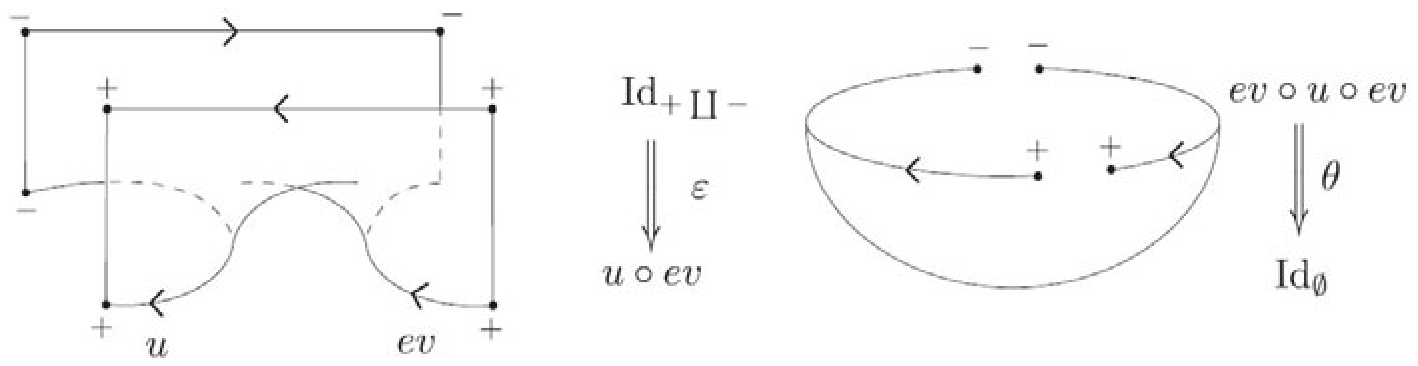
\includegraphics[width=374.4pt]{figs/f3-03.png}
\caption{有向情形下 $u$ 与 $ev$ 的伴随。}
\label{fig:3.3}
\end{figure}

\begin{figure}[htbp]
\centering
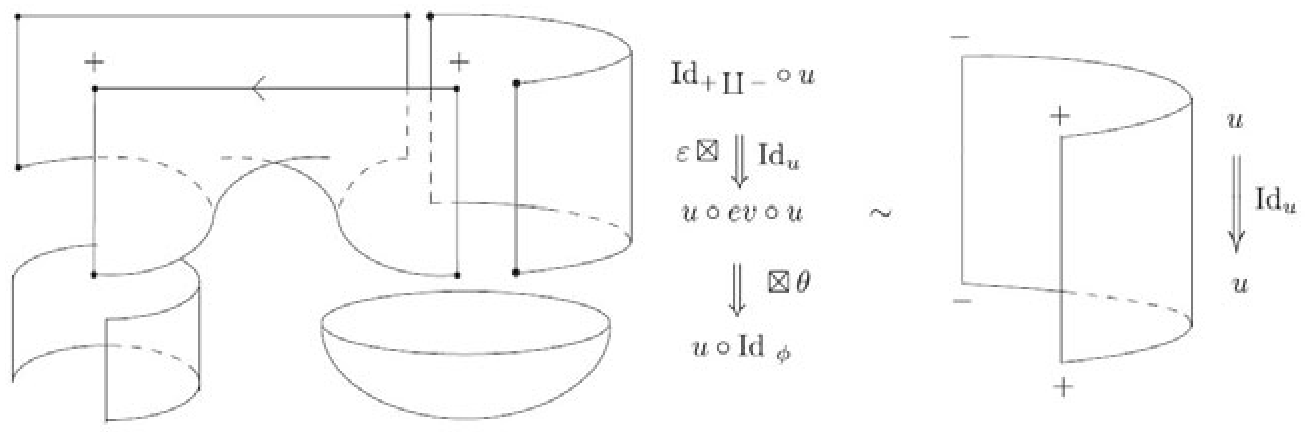
\includegraphics[width=344.5pt]{figs/f3-04.png}
\caption{关系 $(\Id_u\boxtimes\theta)\circ(\varepsilon\boxtimes\Id_u)=\Id_u$。}
\label{fig:3.4}
\end{figure}

这些恒等式「$\theta\circ\varepsilon=1$」正是 Morse 理论中熟知的标准把柄消去关系；图 3.4 与图 3.5 展示了用 2-把柄消去 1-把柄（鞍点）的过程。

\begin{figure}[htbp]
\centering
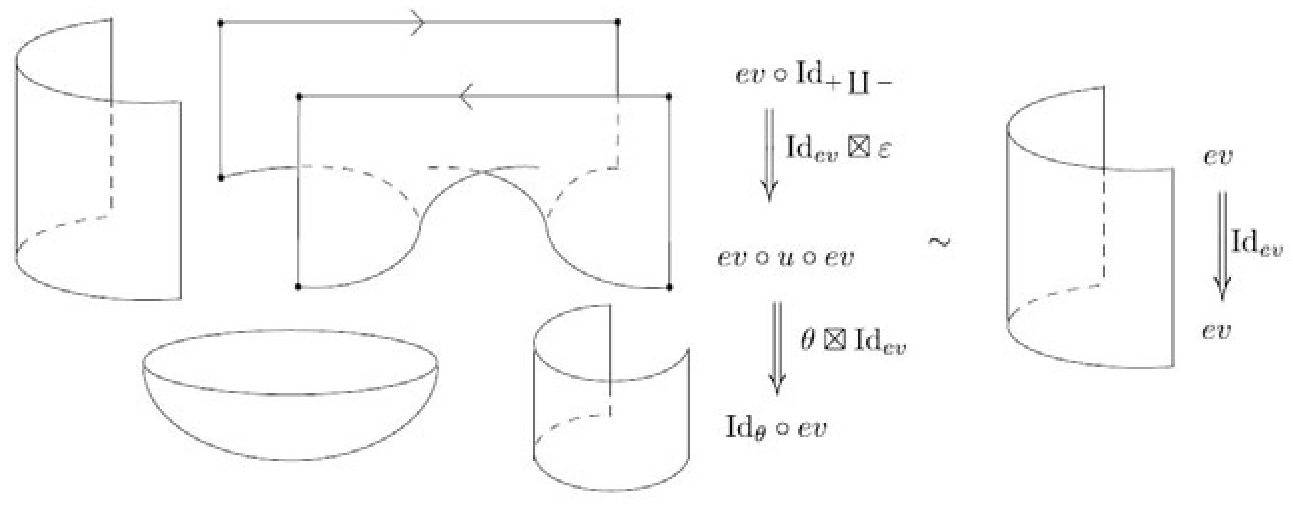
\includegraphics[width=341.4pt]{figs/f3-05.png}
\caption{关系 $(\theta\boxtimes\Id_{ev})\circ(\Id_{ev}\boxtimes\theta)=\Id_{ev}$。}
\label{fig:3.5}
\end{figure}

相反的伴随 $(u,ev)$ 用的是同样的图，但要自下而上读（$\varepsilon$ 与 $\theta$ 的标签也随之互换）。这时 $\varepsilon$ 是 0-把柄，而 $\theta$ 是与之相消的 1-把柄。

\subsection{标架化的把柄}

只要尝试几次，读者便会相信：无法在 1 维把柄 $\supset$ 与 $\subset$ 上放置 2-标架化，使两个伴随 $(ev,u)$ 与 $(u,ev)$ 同时成立。事实上，定义 $u$ 与 $ev$ 时最自然的标架——窄带上的（切向、法向）乘积标架——不允许其中任何一个伴随：这是因为圆盘边界圆周上的径向乘积 2-标架化不能延拓到圆盘内部。我们只好改用 Serre 函子 $S$，它由标准（2-态射、1-态射）乘积标架的一次扭转定义；见图 3.6。

一如既往，我们从右到左读 1-态射、自上而下读 2-态射，正如在源点附近所标示（所以我们的标准标架的定向与页面标架相反）。在所画的带形上，我们取常标架（constant framing）：与乘积标架相比，这多出一次正扭转，并定义了函子 $S$。

现在可以把边界标架延拓到圆盘与鞍点上，以展示伴随对 $\bigl(ev,\,(S\boxtimes\Id_{-})\circ u\bigr)$；一如既往，2-态射自上而下读；见图 3.7（从略）。

与先前相同的把柄消去恒等式照样给出 $\theta\circ\varepsilon=1$。

另一个伴随 $\bigl((S^{-1}\boxtimes\Id_{-})\circ u,\,ev\bigr)$ 则通过自下而上读图得到。（不过我们还必须把边界上竖直方向的 $\R$ 副本变号，以符合源–靶约定；而这一变号会翻转图中的标架扭转。）

\begin{figure}[htbp]
\centering
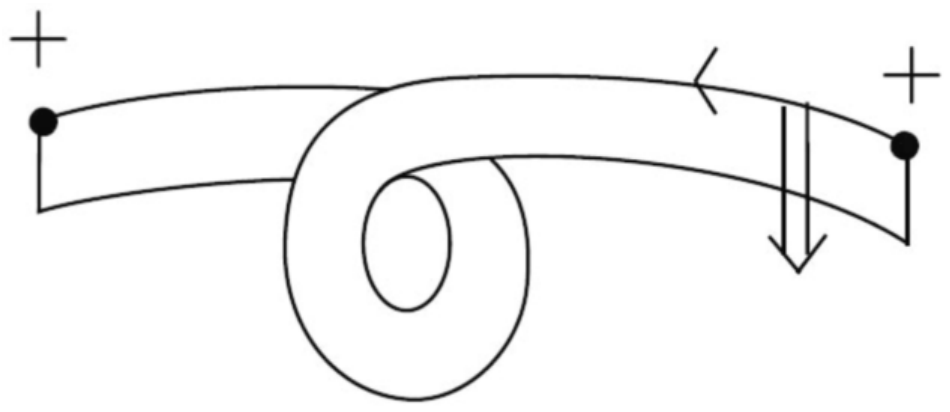
\includegraphics[width=228.0pt]{figs/f3-06.png}
\caption{Serre 函子。}
\label{fig:3.6}
\end{figure}

\begin{figure}[htbp]
\centering
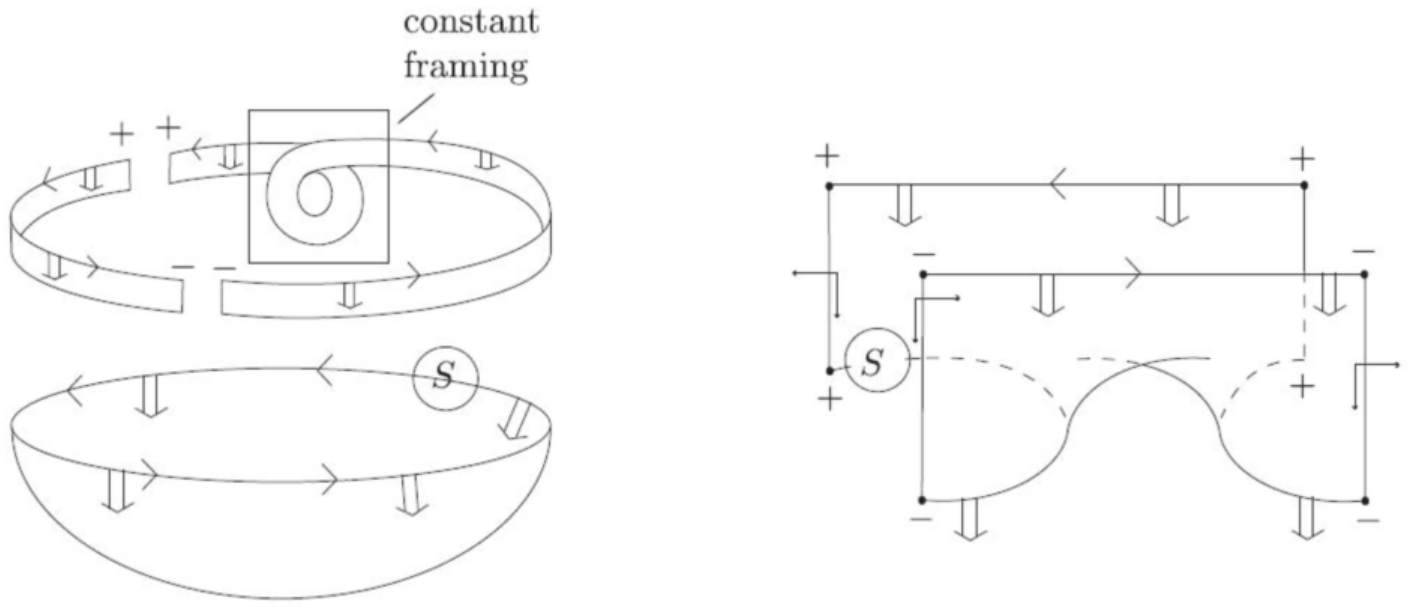
\includegraphics[width=372.2pt]{figs/f3-07.png}
\caption{左：伴随 $ev\circ(S\boxtimes\Id_{-})\circ u\xRightarrow{\ \theta\ }\Id_{\varnothing}$；右：伴随 $\Id_{+\sqcup-}\xRightarrow{\ \varepsilon\ }(S\boxtimes\Id)\circ u\circ ev$。}
\label{fig:3.7}
\end{figure}

\subsection{伴随：代数条件}

为了把伴随条件写开，我们专门考虑由代数、双模（bimodule）与纠缠算子（intertwiner）构成的 2-范畴 $\mathcal{A}\mathrm{lg}$ 这一情形。此时 $\Hom(A,B)$ 是 $(B-A)$-双模的范畴，而态射的复合
\[
\Hom(A,B)\otimes\Hom(B,C)\longrightarrow\Hom(A,C)
\]
由双模在 $B$ 上的张量积给出。\footnote{转换到线性范畴或微分分次范畴的 2-范畴并不困难。微妙的步骤在于幺半结构的定义，即范畴的张量积；对阿贝尔范畴见 [16]。一般地，代数 $A$ 与 $B$ 上的模范畴张量在一起，得到 $(A\otimes B)$-模范畴。}

把这个例子照字面使用过于局限：可以证明，完全可对偶的代数必是半单的。（更一般地，紧生成（compactly generated）阿贝尔范畴在线性范畴中完全可对偶，当且仅当它是半单的，且只有有限多个单同构类。）这仍然富有教益，因为我们将典范地识别出自同构 $S$，并把 $S$ 的平凡化与代数上的 Frobenius 结构或 Calabi--Yau 结构联系起来。然而，要得到更有趣的 TQFT 例子，就必须使用微分分次代数及其模的导出范畴；下面我们回顾射影流形上凝聚层这一例子。

$\mathcal{A}\mathrm{lg}$ 中每个 $A$ 都是可对偶的，其（左与右）对偶是反代数 $A^{\circ}$。事实上，令 $A^{e}:=A\otimes A^{\circ}$；于是可以取空间 $A$ 作为 $u$ 与 $ev$，把它分别视为 $(A^{e}-\C)$-双模与 $(\C-A^{e})$-双模。由此算出 $Z_A(S^1)=A\otimes_{A^{e}}A$，即所谓 $A$ 的第零个 Hochschild 同调（Hochschild homology）。

用 Hom 的定义来计算伴随更为方便。按伴随的 Hom 定义，$u$ 的左伴随 ${}^{\vee}u$ 是一个 $(\C-A^{e})$-双模，满足
\begin{equation}
\Hom_{A^{e}}(M,\,A\otimes_{\C}N)=\Hom_{\C}({}^{\vee}u\otimes_{A^{e}}M,\,N)
\tag{3.7}\label{eq:3.7}
\end{equation}
对任意 $A^{e}$-模 $M$ 与任意 $\C$-向量空间 $N$。（其实，我们应当要求这对任意代数 $B$ 以及 $N$ 上的右 $B$-模结构都成立；但后者会自动得到。）先取 $M=A^{e}$、$N=\C$，再要求它对任意 $N$ 成立，便导出条件 $A=\Hom_{\C}({}^{\vee}u,\C)$ 与 $\dim_{\C}{}^{\vee}u<\infty$；于是 $\dim A<\infty$，且 ${}^{\vee}u=A^{\vee}:=\Hom(A,\C)$，即 $A$ 的对偶向量空间。此外，要使 (3.7) 对所有 $M$ 成立，还需要 $M\mapsto A^{\vee}\otimes_{A^{e}}M$ 的左正合性，即 $A^{\vee}$ 的 $A^{e}$-平坦性。

\begin{exercise}
证明：作为推论，有限维 $A$-模的范畴是半单的，因而 $A$ 是半单的。（由此推出有限维 $A$-模的范畴中 $\Hom$ 的正合性。）
\end{exercise}

继续下去，由于 $ev^{\vee}=(S\boxtimes\Id)\circ u$，必须有 $ev={}^{\vee}u\circ(S^{-1}\boxtimes\Id)$；于是我们断定：$S$ 典范地就是 $(A-A)$-双模 $A^{\vee}$，而且它必须是可逆双模。其次，对左伴随 ${}^{\vee}ev$，有
\begin{equation}
\Hom_{A^{e}}({}^{\vee}ev\otimes_{\C}M,\,N)=\Hom_{\C}(M,\,A\otimes_{A^{e}}N)
\tag{3.8}\label{eq:3.8}
\end{equation}
由此，取 $M=\C$、$N=A^{e}$，便得到 $A=\Hom_{A^{e}}({}^{\vee}ev,A^{e})$。此外，要一般地还原同构 (3.8)，需要 $A$ 在 $A^{e}$ 上的平坦性与有限展示性。其余伴随的存在不再提供任何信息或限制：$u^{\vee}=\Hom_{A^{e}}(A,A^{e})={}^{\vee}ev$，而 $ev^{\vee}=A^{\vee}={}^{\vee}u$。

\begin{remark}
$S$ 是 $A$ 的向量空间对偶，这并非偶然；见 §3.5.5。
\end{remark}

若改用微分分次代数，并以拟同构代替等式，则 $A$ 的有限维性变成 $A$ 的同调的有限性，通常称为紧性（compactness）；而 $A$ 在 $A^{e}$ 上的有限性则是光滑性（smoothness）。这是因为它们分别与复簇情形中的相应性质吻合。用这套语言，完全可对偶的 dga 就是紧且光滑的那些；这一点或许最早在 Kontsevich--Soibelman [18] 的工作中被指出。

\subsection{由 Frobenius 代数得到定向 TQFT}

Serre 函子的一个平凡化是 $A^{e}$-模同构 $A\cong A^{\vee}$。在这一等同下，$1$ 的像定义了一个线性映射 $t\colon A\to\C$，它诱导出对称非退化迹 $a\times b\mapsto t(ab)=t(ba)$，从而使 $A$ 成为一个非交换 Frobenius 代数。\begin{annote}底本此处作 $t\colon a\to\C$，小写 $a$ 与上下文不合，当为 $A$ 之误；译文按 $A$ 写出。（来源：底本印刷页 149；应登记疑点清单）\end{annote}

借助 $t$，我们可以把 $Z_A(S^1)=ev\circ u=\Hom(A\otimes_{A^{e}}A;\C)$ 的对偶空间与 $Z(A)=\Hom_{A^{e}}(A,A^{\vee})\cong\Hom_{A^{e}}(A,A)$（即 $A$ 的中心）等同起来。后者同样是半单交换代数，并从伴随的余单位 $\theta\colon Z_A(S^1)\to\C$ 获得 Frobenius 结构。包含映射 $Z(A)\to A$ 是代数同态，而投影 $A\to Z_A(S^1)$ 可用来借助 $\theta$ 分解 $A$ 上的迹 $t$。Moore--Segal [22] 极为详细地讨论了这些例子，它们启发了其后的许多工作 [7, 18]。

结论：2 维扩张定向 TQFT 恰好对应于半单但不必交换的 Frobenius 代数。

\subsection{有限规范理论再访}

沿用 [22] 的做法，令 $A$ 为有限群的群环 $\C\langle F\rangle$；我们选取迹 $t\colon\C\langle F\rangle\to\C$，以挑出 $1$ 的系数。显式地，配对为
\[
t(\varphi\cdot\psi)=\sum_{f\in F}\varphi(f)\psi(f^{-1}).
\]

我断言：$Z$ 就是带角曲面的 $F$-规范理论（事实上，它是一个无定向 TQFT）。该理论在 1-流形上是显然的：把区间送到 $A=\C\langle F\rangle$，把圆周送到 $Z(A)$，即 $F$ 上的类函数。它在曲面上仍由「计数 $F$-丛、并按自同构加权」来定义；与 §3.1 的 $(1,2)$-理论不同之处在于：现在丛在角上被平凡化（在界定 2-态射的恒等线段上也被平凡化）。

\begin{exercise}
把上述定义精确化，并验证它给出一个从 $\mathsf{Bord}^{\mathrm{O}(2)}_{2}$ 到 $\mathcal{A}\mathrm{lg}$ 的函子。
\end{exercise}

\begin{remark}
迹 $t$ 可自然地延拓到 $F$-表示的整个范畴 $\mathrm{Rep}(F)$：对表示范畴中任意对象 $V$，定义 $t_V=(\#F)^{-1}\operatorname{Tr}_V\colon\operatorname{End}^{G}(V)\to\C$。迹性质是 $t(\varphi\circ\psi)=t(\psi\circ\varphi)$，对任意一对源与靶相反的态射成立。这就对所有的 $V,W$ 定义了 $\Hom^{G}(V,W)$ 与 $\Hom^{G}(W,V)$ 之间的非退化配对，并给出 $\mathrm{Rep}(F)$ 上 Calabi--Yau 结构的一个例子：该范畴上 Serre 函子的一个平凡化——我们接下来将在簇的语境中考察它。它还提供了开–闭理论（open--closed theory，相关定义见 [7]）的一个例子，其中 $\mathrm{Rep}(F)$ 是膜（brane）范畴。
\end{remark}

\subsection{概形上的 Serre 函子}

在研究射影流形 $X$ 上凝聚层的导出范畴时，Bondal 与 Orlov 指出了 Serre 自同构（Serre automorphism）的作用；在任何线性范畴 $\mathcal{C}$ 中，它由存在双函子同构
\[
\Hom(x,S(y))=\Hom(y,x)^{\vee}
\]
来刻画。

若它存在，则 $S\colon\mathcal{C}\to\mathcal{C}$ 在典范同构的意义下唯一。若 $S$ 可逆，则它迫使各 $\Hom$ 空间与其双重对偶同构，从而是有限维的；这是一个很强的条件。若再假设 $\mathcal{C}$ 紧生成（一个较温和的有限性条件），则可证明 $\mathcal{C}$ 是线性范畴 2-范畴中的 2-可对偶对象，从而定义一个标架化的 2 维 TQFT。此外，上面定义的 Serre 函子与由标架扭转定义的那个一致。

在导出范畴的情形，取层复形之间的第零个群 $\operatorname{Ext}^{0}(\mathcal{F}^{\bullet},\mathcal{G}^{\bullet})$ 作为 Hom，Serre 的经典对偶定理便把 $S$ 等同于与 $K_X[\dim X]$ 作张量的函子，即把典范丛平移至次数 $(-\dim X)$。下面这个结果是配边假设的一个非凡应用；Calabi--Yau 情形曾以略有不同的形式，由 Costello [7] 与 Kontsevich 独立证明。

\begin{theorem}
射影流形 $X$ 上（有界）凝聚层复形的导出范畴 $D^{b}\mathrm{Coh}(X)$ 是完全可对偶的。Serre 函子是顺时针的标架扭转。要定义一个定向 TQFT，需要 $X$ 上的 Calabi--Yau 结构：典范丛的一个平凡化。
\end{theorem}

这是对半单情形的巨大推广；后者在 $X$ 为有限集时得到。

\subsection{联系于圆周的向量空间}

让我们在 $\mathcal{C}=\mathrm{Coh}(X)$ 的情形理解 $Z(S^1)$。当 $D=1$ 时，圆周算出一个数，即向量空间的维数。可见我们是在把维数的概念推广到线性范畴，而得到的答案是一个向量空间。

在标架化的语境中，圆周有许多个 $S^1_n$，对每个整数 $n$ 各一个，计数 2-标架化绕圆周的绕数。于是我们的 TQFT 对每个 $n\in\Z$ 都有一个态空间 $Z(S^1_n)$。我们用 $0$ 标记 $\R^{2}$ 中标准单位圆盘所界定的那个圆周标架。若把两个半圆粘在一起来构造 $S^1_n$，则这些圆周之间的差别在于：在粘合之前插入 Serre 自同构的幂次。按我们的约定，
\[
Z(S^1_0)=ev\circ(S^{-1}\boxtimes\Id_{-})\circ u,
\qquad
Z(S^1_1)=ev\circ u,
\]
后者是维数的直接类比。

\begin{theorem}
当 $Z(+)=D^{b}\mathrm{Coh}(X)$ 时，$Z(S^1_n)=H^{*}\bigl(X;\,K^{\otimes n}\otimes\Lambda^{*}(T_X)\bigr)$。
\end{theorem}

\begin{remark}
对 $n=0$，这是流形 $X$ 的 Hochschild 上同调；对 $n=1$，它是 Hochschild 同调。上同调带有自然的环结构，而同调是它上面的模（其余空间亦然）。这个代数结构正是由 TQFT 中裤子态射 $S^1_0\sqcup S^1_0\to S^1_0$ 所描述的，其标架化通过把它实现为 $\R^2$ 中嵌入一个大圆盘的两个较小圆盘而得到。离开 Calabi--Yau 情形就没有 Frobenius 代数结构，因为迹（即出向的标架化圆盘）来自配边 $S^1_2\to\varnothing$。不过存在配对 $S^1_1\sqcup S^1_1\to S^1_2$，再从它走到 $\varnothing$，便在 Hochschild 同调上给出一个完美双线性配对。
\end{remark}
